\documentclass[11pt,a4paper]{scrartcl}
\usepackage[utf8]{inputenc}
\usepackage[spanish,es-noshorthands]{babel}
\usepackage[margin=2.5cm]{geometry}
\usepackage{graphicx}
\usepackage{amsmath}
\usepackage{booktabs}
\usepackage{float}
\usepackage[hidelinks]{hyperref}

\newcommand{\sig}[1]{\texttt{#1}}

\title{Diseño digital avanzado}
\subtitle{Trabajo práctico 1: shift register de LEDs}
\author{Krede, Julian}
\date{\today}

\begin{document}
	\maketitle

	\begin{abstract}
		Se describe el diseño de un shift register circular que enciende los LEDs de la placa
		Arty A7 de a uno por vez, con velocidad, habilitación y color seleccionables mediante
		switches. El diseño incluye un VIO para manejar las entradas en forma remota y un ILA
		para observar las salidas. Se verificó por simulación y se implementó en una FPGA del
		cluster remoto.
	\end{abstract}

	% ------------------------------------------------------------------
	\section{Diseño}

	El sistema enciende un LED a la vez y desplaza el bit encendido en forma circular
	($0001 \to 0010 \to 0100 \to 1000 \to 0001 \dots$). Un contador marca cada cuánto se
	desplaza. Las entradas son:

	\begin{itemize}
		\item \sig{i\_reset}: reset del sistema (botón \sig{ck\_rst}, activo en bajo). Pone a cero
		el contador e inicializa el shift register en \sig{0001}.
		\item \sig{i\_sw[0]}: habilitación. Con 0 el sistema se detiene sin perder el estado del
		contador ni del shift register.
		\item \sig{i\_sw[2:1]}: selección del límite del contador R0--R3, es decir, de la velocidad.
		\item \sig{i\_sw[3]}: color de los LEDs RGB (0 azul, 1 verde).
	\end{itemize}

	La Figura~\ref{fig:top} muestra la arquitectura del módulo \sig{top}, que se dividió en
	dos módulos (\sig{count} y \sig{shiftreg}) más la lógica de selección de entradas y de
	color.

	\begin{figure}[H]
		\centering
		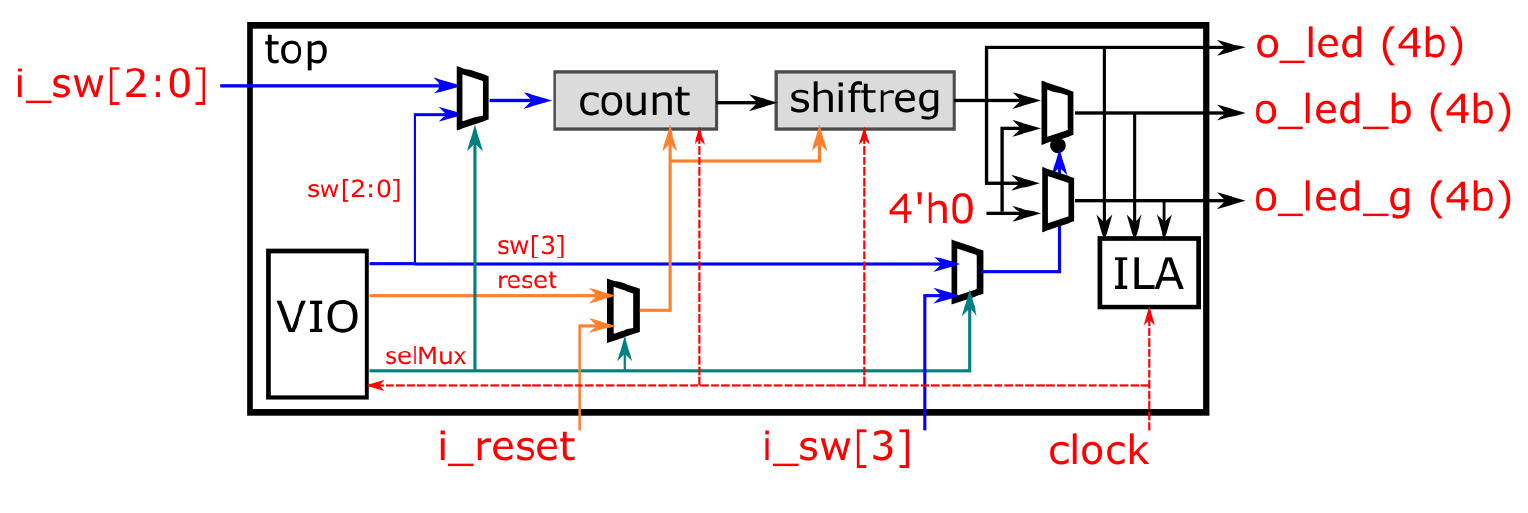
\includegraphics[width=0.95\textwidth]{figuras/diagrama_top.png}
		\caption{Diagrama en bloques del módulo \sig{top}.}
		\label{fig:top}
	\end{figure}

	\subsection{Contador (\sig{count.v})}

	Es un contador de \sig{NB\_COUNTER} = 32 bits con reset asincrónico activo en alto. Un
	multiplexor elige el límite según \sig{i\_sel} (\sig{i\_sw[2:1]}):
	\[
		R_k = 2^{\,N_{c} - 10 + k} - 1, \qquad k = 0,\dots,3 ,
	\]
	donde $N_c$ es la cantidad de bits del contador. En cada flanco, si \sig{i\_enable = 1}:

	\begin{itemize}
		\item si el contador llegó al límite (\sig{counter >= ref\_limit}) vuelve a cero;
		\item si no, se incrementa en uno.
	\end{itemize}

	Con \sig{i\_enable = 0} mantiene el valor. La salida
	\[
		\sig{o\_valid = i\_enable \& (counter >= ref\_limit)}
	\]
	vale 1 durante el ciclo en que el contador está en el límite y es la que habilita el
	desplazamiento.

	Se comparó con \sig{>=} en lugar de \sig{==} porque el límite puede cambiarse en
	cualquier momento. Si el contador está, por ejemplo, en $2^{24}$ y se pasa a R0
	($2^{22}-1$), con \sig{==} tendría que dar la vuelta completa de $2^{32}$ cuentas (unos
	43\,s) hasta volver a pasar por el límite. Con \sig{>=}, en cambio, se reinicia en el
	ciclo siguiente.

	\paragraph{Tiempo entre desplazamientos.} El contador recorre los valores $0, 1, \dots, R_k$
	y vuelve a 0, así que hay un desplazamiento cada $R_k + 1 = 2^{\,N_c-10+k}$ ciclos. Con el
	reloj de 100\,MHz ($T_{clk} = 10$\,ns) y $N_c = 32$:
	\[
		T_k = (R_k + 1)\, T_{clk} = 2^{\,22+k} \cdot 10\,\text{ns} .
	\]

	\begin{table}[H]
		\centering
		\begin{tabular}{@{}cccc@{}}
			\toprule
			\sig{i\_sw[2:1]} & Límite & Ciclos por paso & Tiempo por paso \\
			\midrule
			\sig{00} & $R_0 = 2^{22}-1$ & $2^{22}$ & $\approx 42$\,ms \\
			\sig{01} & $R_1 = 2^{23}-1$ & $2^{23}$ & $\approx 84$\,ms \\
			\sig{10} & $R_2 = 2^{24}-1$ & $2^{24}$ & $\approx 168$\,ms \\
			\sig{11} & $R_3 = 2^{25}-1$ & $2^{25}$ & $\approx 336$\,ms \\
			\bottomrule
		\end{tabular}
	\end{table}

	Cada código de \sig{i\_sw[2:1]} duplica el tiempo del anterior. El límite más grande
	necesita 25 bits, así que el contador de 32 bits alcanza con margen.

	\subsection{Shift register (\sig{shiftreg.v})}

	Es un registro de \sig{N\_LEDS} = 4 bits con reset asincrónico activo en alto, que lo
	inicializa en \sig{0001}. Cuando \sig{i\_valid = 1} rota un lugar a la izquierda, y el
	bit más significativo vuelve a la posición 0:
	\[
		\sig{shiftreg} \leftarrow \{\sig{shiftreg[2:0]},\ \sig{shiftreg[3]}\} .
	\]
	Como \sig{i\_valid} es el \sig{o\_valid} del contador, el registro se desplaza una sola
	vez cada $T_k$, y se queda quieto cuando el sistema está deshabilitado.

	\subsection{Módulo principal (\sig{top.v})}

	\begin{itemize}
		\item \textbf{Selección placa / VIO.} La salida \sig{selMux} del VIO elige de dónde se
		toman los switches y el reset: de los pines de la placa (\sig{selMux = 0}) o de las
		salidas del VIO (\sig{selMux = 1}). Esto permite manejar el diseño sin acceso físico a
		la placa.
		\item \textbf{Reset.} Tanto \sig{ck\_rst} como el reset del VIO son activos en bajo; en el
		\sig{top} se invierten para generar el \sig{reset} interno activo en alto que usan
		\sig{count} y \sig{shiftreg}.
		\item \textbf{Color.} Dos multiplexores mandan el estado del shift register al canal azul
		(\sig{o\_led\_b}) si \sig{sw[3] = 0}, o al verde (\sig{o\_led\_g}) si \sig{sw[3] = 1}; el
		otro canal recibe \sig{4'h0}. Los LEDs simples \sig{o\_led} siempre muestran el estado.
		\item \textbf{Debug.} El VIO y el ILA observan las señales internas \sig{connect\_leds},
		\sig{led\_b} y \sig{led\_g}, ya que no es posible conectar un IP a un puerto de salida.
	\end{itemize}

	\subsection{Constraints}

	El archivo \sig{Arty\_Master\_v2.xdc} asigna los pines de la placa: el reloj de 100\,MHz
	(\sig{E3}) con su \sig{create\_clock} de 10\,ns, los switches SW0--SW3 a \sig{i\_sw[3:0]},
	el botón \sig{ck\_rst} a \sig{i\_reset}, los canales azul y verde de los LEDs RGB
	LD0--LD3 a \sig{o\_led\_b} y \sig{o\_led\_g}, y los LEDs LD4--LD7 a \sig{o\_led}.

	% ------------------------------------------------------------------
	\section{Simulación}

	El testbench \sig{tb\_shiftleds.v} instancia el \sig{top} sin los IP cores, como pide el
	enunciado. Como en simulación nadie maneja el VIO, se fuerza
	\sig{selMux = 0} con \sig{force} para que las entradas se tomen de la placa.

	Para que la simulación no tarde demasiado, el contador se parametrizó con
	\sig{NB\_COUNT = 14}. Con la fórmula anterior los límites quedan
	\[
		R_k + 1 = 2^{\,14-10+k} = 2^{\,4+k} = 16,\ 32,\ 64,\ 128 \text{ ciclos}
		\quad\Rightarrow\quad T_k = 160,\ 320,\ 640,\ 1280\ \text{ns} .
	\]

	Secuencia de estímulos:

	\begin{enumerate}
		\item Reset activo durante 100\,ns y luego se libera.
		\item Se habilita el sistema (\sig{sw[0] = 1}) con \sig{sw[2:1] = 00}.
		\item Cada 1\,ms se cambia la configuración: \sig{sw[2:1] = 01}, luego \sig{10}, luego
		\sig{sw[3] = 1} (verde) y por último \sig{sw[2:1] = 11}.
	\end{enumerate}

	\subsection{Resultados}

	En la Figura~\ref{fig:vel} se ve un tramo de cada configuración. El LED encendido rota
	$0 \to 1 \to 2 \to 3 \to 0$ y cada desplazamiento coincide con un pulso de un ciclo de
	\sig{o\_valid}. Midiendo el tiempo entre desplazamientos en toda la simulación se obtuvo
	exactamente 160, 320, 640 y 1280\,ns para cada código, es decir $2^{4+k}$ ciclos, como se
	calculó. También se cumplió después de cada cambio de límite.

	\begin{figure}[H]
		\centering
		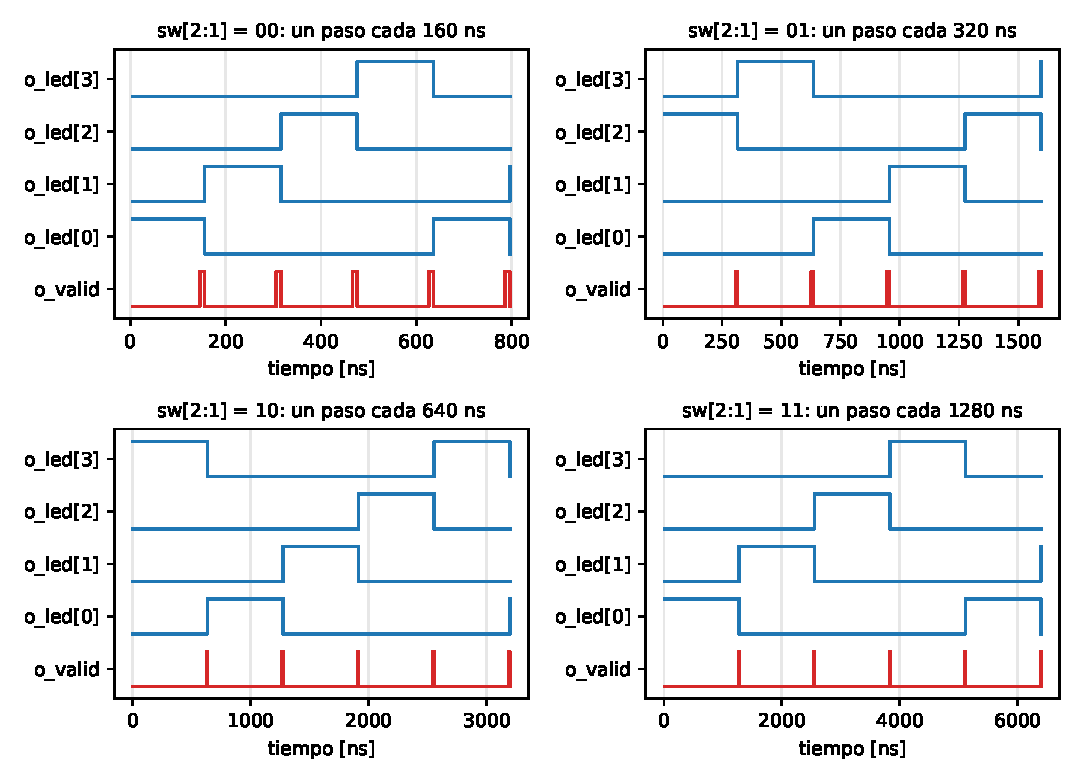
\includegraphics[width=\textwidth]{figuras/tb_velocidades.pdf}
		\caption{Simulación: estado del shift register y \sig{o\_valid} para cada límite.}
		\label{fig:vel}
	\end{figure}

	En la Figura~\ref{fig:color} se ve el cambio de color en $t = 3$\,ms. Antes de que
	\sig{sw[3]} pase a 1, el estado se muestra en \sig{o\_led\_b} y \sig{o\_led\_g} está en
	cero; después pasa a \sig{o\_led\_g} y el canal azul se apaga. El shift register no
	pierde su posición, porque el color solo afecta a los multiplexores de salida.

	\begin{figure}[H]
		\centering
		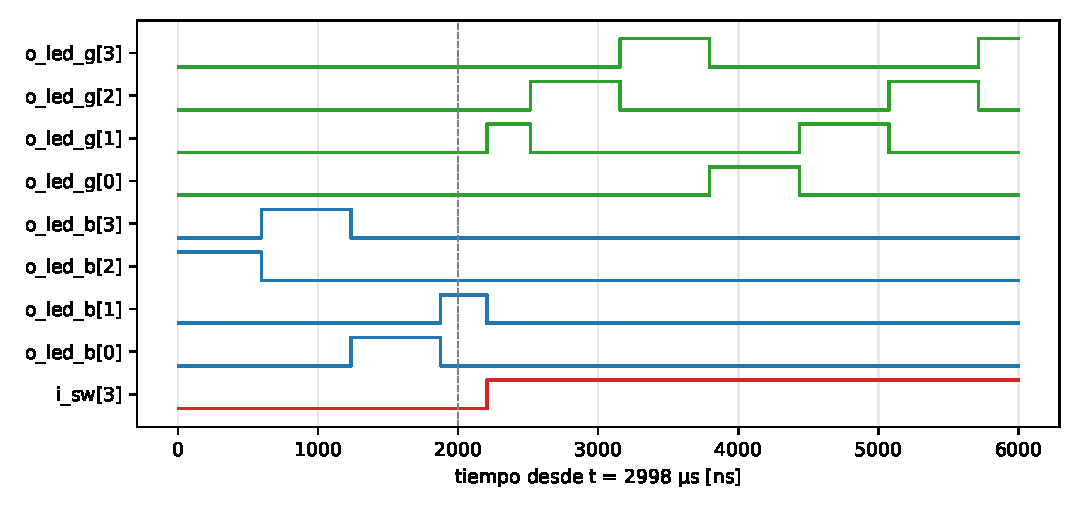
\includegraphics[width=\textwidth]{figuras/tb_color.pdf}
		\caption{Simulación: cambio de color con \sig{sw[3]} (línea punteada).}
		\label{fig:color}
	\end{figure}

	% ------------------------------------------------------------------
	\section{Implementación en la FPGA}

	Como no se tiene acceso físico a la placa, el diseño se implementó en una Arty A7 de un
	cluster remoto, y para manejarlo y observarlo se agregaron dos IP cores:

	\begin{itemize}
		\item \textbf{VIO}, con 3 entradas de 4 bits (\sig{connect\_leds}, \sig{led\_b},
		\sig{led\_g}) para ver el estado, y 3 salidas: \sig{selMux} (1 bit), el reset
		(1 bit, activo en bajo) y los switches (4 bits). Al pasar a \sig{selMux = 1} hay que
		poner el reset del VIO en 1; si queda en 0 el sistema se mantiene en reset.
		\item \textbf{ILA}, con 3 probes de 4 bits conectados a las mismas señales internas,
		para capturar las formas de onda con el reloj del sistema.
	\end{itemize}

	El flujo fue: crear el proyecto en Vivado para la Arty A7 con los archivos de \sig{src/}
	y \sig{constrains/}, agregar los IP \sig{vio} e \sig{ila} con esa configuración,
	sintetizar, implementar y generar el bitstream. Después, conectarse por SSH al servidor
	del cluster, solicitar una FPGA, agregar en el Hardware Manager de Vivado el
	\emph{remote server} con la IP asignada, y programar la placa. Luego, mediante el VIO y el
	ILA, se analizó el funcionamiento del diseño implementado en la placa.
\end{document}
